\section{Examples}
\label{sec:examples}
We implemented the above smooth approximation to the semantics of MTL, and tested them empirically on a number of examples.

\subsection{Approximation error}
\label{sec: ex apx error}
\begin{figure}[t]
\centering
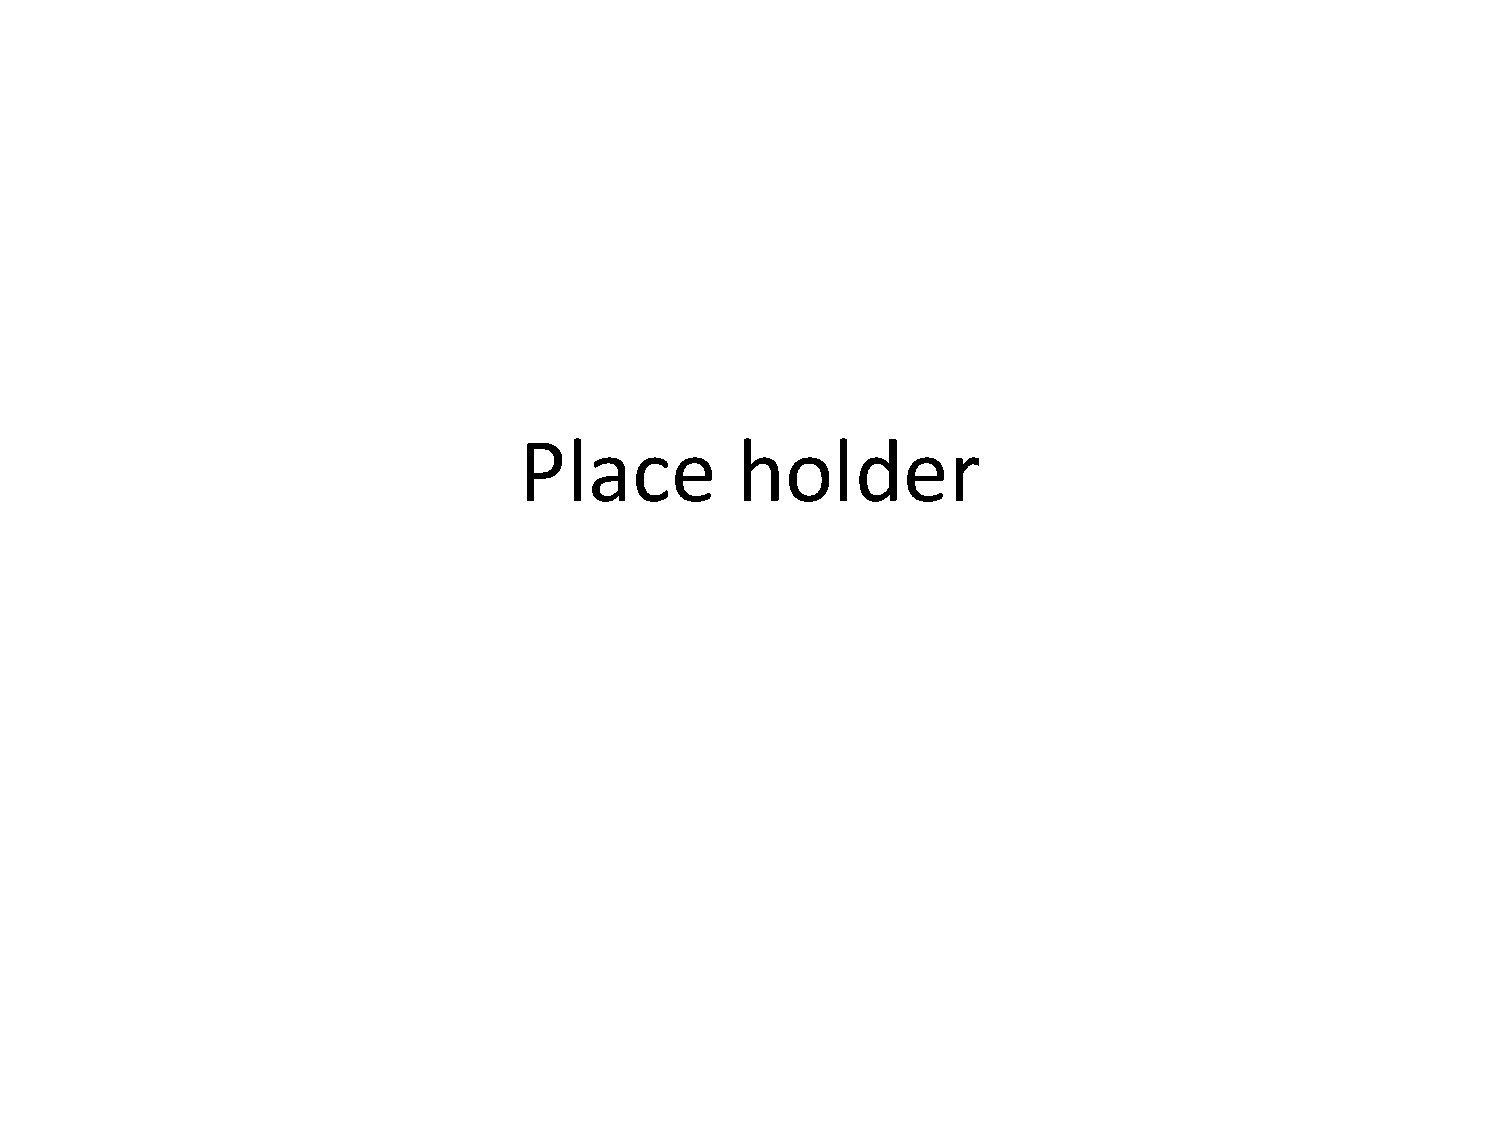
\includegraphics[width=0.7\linewidth]{figures/placeHolder}
\caption{Relative approximation error (left) and smooth approximation of distance function for ??? (right)}
\label{fig:sample result}
\end{figure}
\todo[inline]{Yash, Show these results}
We first meaured the actual approximation error over several examples.
The results are presented in Table \ref{tab:ex apx error}.
It can be seen that ???
Fig. \ref{fig:sample result} shows the relative absolute approximation error.
???

\subsection{Robustness maximization for control}
\label{sec:toy example}
\todo[inline]{Yash, Show SA and SR-SQP on toy example}

\subsection{Robustness minimization for falsification}
\label{sec:toy falsification}
\todo[inline]{Yash, Show the falsification figure for an autonomous system, comparing Method, DumbSqp,SA}
